%
% projektiv.tex
%
% (c) 2017 Prof Dr Andreas Müller, Hochschule Rapperswil
%
\subsection{Kleinsche Flasche}
Eine Kleinsche Flasche ist eine Fläche, die sich selbst durchdringt.
Die Fläche hat nur ein Seite und keinen Rand.
Wir können die Fläche mit einem Netzwerk von Dreiecken überziehen
und die Homologievektorräume berechnen oder mindestens deren Dimensionen
berechnen.
Dies ist jedoch einfacher, wenn man die Kleinsche Flasche aus einfacheren
Flächen zusammensetzen, die entsprechend einfachere Dreiecksnetze
haben.

Ein Möbius-Band entsteht, wenn man eine Streifen Papier eine halbe 
Drehung verdreht zusammenklebt.
Das Möbiusband hat nur eine Seite und nur eine Kante.
Man kann also ein Möbius-Band entlang dieses Randes mit einer
Kreisscheibe zusammenkleben.
Es stellt sich heraus, dass dadurch eine Kleinsche Flasche entsteht.
Der Plan ist also, eine Triangulation von Kreisscheibe und Möbiusband
zu finden, die am Rande zusammenpassen.
Daraus können wir dann die Randoperatoren und letztlich die Betti-Zahlen
berechnen.

\begin{figure}
\centering
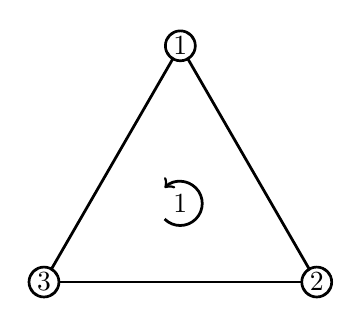
\begin{tikzpicture}[scale=4]
\coordinate (A) at (0,0.5);
\coordinate (B) at (0.433,-0.25);
\coordinate (C) at (-0.433,-0.25);
\draw[line width=1pt] (A)--(B);
\draw[line width=1pt] (A)--(C);
\draw[line width=1pt] (B)--(C);
\draw[fill=black] (A) circle[radius=0.5mm,fill]{};
\draw[fill=white] (A) circle[radius=0.45mm,fill]{};
\node at (A) {$1$};
\draw[fill=black] (B) circle[radius=0.5mm,fill]{};
\draw[fill=white] (B) circle[radius=0.45mm,fill]{};
\node at (B) {$2$};
\draw[fill=black] (C) circle[radius=0.5mm,fill]{};
\draw[fill=white] (C) circle[radius=0.45mm,fill]{};
\node at (C) {$3$};
\node at (0,0) {$1$};
\draw[->,line width=1pt] (-0.5mm,-0.5mm)
	arc[x radius=0.7mm,y radius=0.7mm,start angle=-135,end angle=135];
\end{tikzpicture}
\caption{Triangulation der Kreisscheibe
\label{homologie:fig:disk}}
\end{figure}

\begin{figure}
\centering
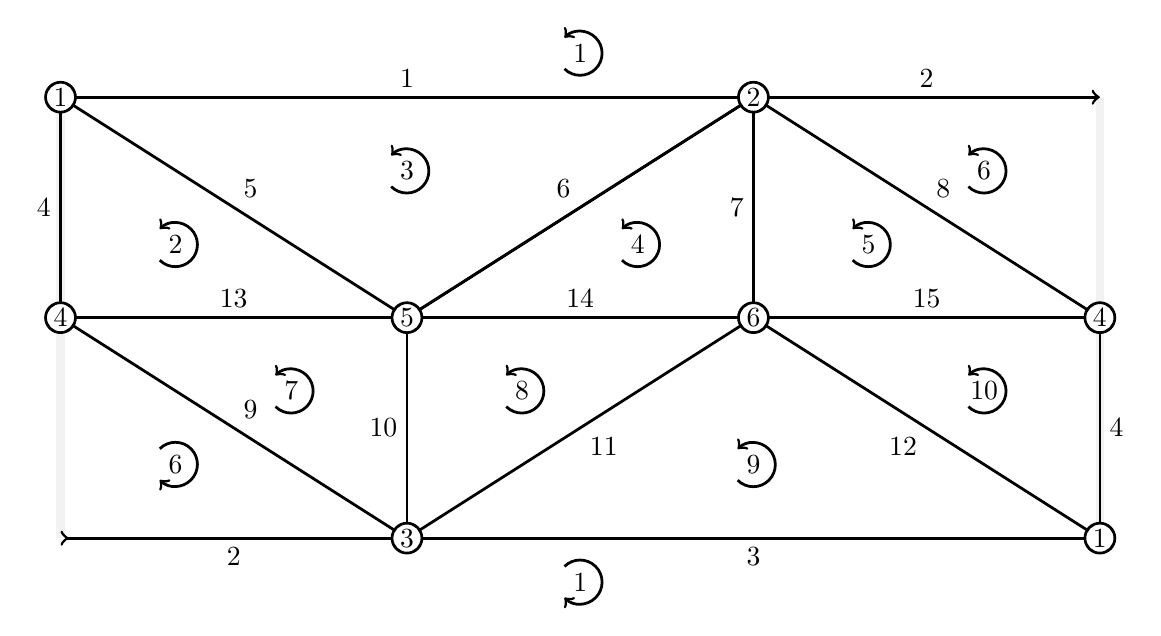
\begin{tikzpicture}[scale=4]
\def\w{2.2}
\def\h{1.4}
\coordinate (A) at ({0 * \w},{0.5 * \h});
\coordinate (a) at ({1.5 * \w},{-0.5 * \h});
\coordinate (B) at ({1 * \w},{0.5 * \h});
\coordinate (C) at ({0.5 * \w},{-0.5 * \h});
\coordinate (D) at ({0 * \w},{0 * \h});
\coordinate (E) at ({0.5 * \w},{0 * \h});
\coordinate (F) at ({1 * \w},{0 * \h});
\coordinate (d) at ({1.5 * \w},{0 * \h});
\draw[line width=3pt,color=gray!10] (A)--({0 * \w},{-0.5 * \h});
\draw[line width=3pt,color=gray!10] (a)--({1.5 * \w},{0.5 * \h});

\draw[->,line width=1pt] (A)--({1.5 * \w},{0.5 * \h});
\draw[>-,line width=1pt] ({0 * \w},{-0.5 * \h})--(a);

\draw[line width=1pt] (A)--(D);
\draw[line width=1pt] (A)--(E);
\draw[line width=1pt] (D)--(E);

\draw[line width=1pt] (B)--(E);
\draw[line width=1pt] (B)--(F);
\draw[line width=1pt] (E)--(F);

\draw[line width=1pt] (B)--(E);
\draw[line width=1pt] (B)--(d);
\draw[line width=1pt] (E)--(d);

\draw[line width=1pt] (D)--(C);
\draw[line width=1pt] (E)--(C);

\draw[line width=1pt] (C)--(F);
\draw[line width=1pt] (F)--(a);

\draw[line width=1pt] (a)--(d);

\draw[fill=black] (A) circle[radius=0.5mm,fill]{};
\draw[fill=white] (A) circle[radius=0.45mm,fill]{};
\node at (A) {$1$};

\draw[fill=black] (B) circle[radius=0.5mm,fill]{};
\draw[fill=white] (B) circle[radius=0.45mm,fill]{};
\node at (B) {$2$};

\draw[fill=black] (C) circle[radius=0.5mm,fill]{};
\draw[fill=white] (C) circle[radius=0.45mm,fill]{};
\node at (C) {$3$};

\draw[fill=black] (a) circle[radius=0.5mm,fill]{};
\draw[fill=white] (a) circle[radius=0.45mm,fill]{};
\node at (a) {$1$};

\draw[fill=black] (D) circle[radius=0.5mm,fill]{};
\draw[fill=white] (D) circle[radius=0.45mm,fill]{};
\node at (D) {$4$};

\draw[fill=black] (E) circle[radius=0.5mm,fill]{};
\draw[fill=white] (E) circle[radius=0.45mm,fill]{};
\node at (E) {$5$};

\draw[fill=black] (F) circle[radius=0.5mm,fill]{};
\draw[fill=white] (F) circle[radius=0.45mm,fill]{};
\node at (F) {$6$};

\draw[fill=black] (d) circle[radius=0.5mm,fill]{};
\draw[fill=white] (d) circle[radius=0.45mm,fill]{};
\node at (d) {$4$};

\def\flaeche#1#2{%
\node at #1 {#2};
\draw[->,line width=1pt] #1 + (-0.5mm,-0.5mm)
	arc[x radius=0.7mm,y radius=0.7mm,start angle=-135,end angle=135];
}

\def\rflaeche#1#2{%
\node at #1 {#2};
\draw[->,line width=1pt] #1 + (-0.5mm,0.5mm)
	arc[x radius=0.7mm,y radius=0.7mm,start angle=135,end angle=-135];
}

\flaeche{({0.166*\w},{0.166*\h})}{$2$};
\flaeche{({0.5*\w},{0.333*\h})}{$3$};
\flaeche{({0.833*\w},{0.166*\h})}{$4$};
\flaeche{({1.166*\w},{0.166*\h})}{$5$};
\flaeche{({1.333*\w},{0.333*\h})}{$6$};
\flaeche{({0.333*\w},{-0.166*\h})}{$7$};
\flaeche{({0.666*\w},{-0.166*\h})}{$8$};
\flaeche{({1*\w},{-0.333*\h})}{$9$};
\flaeche{({1.333*\w},{-0.166*\h})}{$10$};

\rflaeche{({0.166*\w},{-0.333*\h})}{$6$};
%\node at ({0.166*\w},{-0.333*\h}) {$6$};
%\draw[->,line width=1pt]
%	({0.166*\w},{-0.333*\h}) +(-0.5mm,0.5mm)
%	arc[x radius=0.7mm,y radius=0.7mm,start angle=135,end angle=-135];

\flaeche{({0.75*\w},{0.6*\h})}{$1$};
\rflaeche{({0.75*\w},{-0.6*\h})}{$1$};

\node at ({0.5*\w},{0.5*\h}) [above] {$1$};
\node at ({1.25*\w},{0.5*\h}) [above] {$2$};
\node at ({1*\w},{-0.5*\h}) [below] {$3$};
\node at ({0.25*\w},{-0.5*\h}) [below] {$2$};

\node at ({0*\w},{0.25*\h}) [left] {$4$};
\node at ({0.25*\w},{0.25*\h}) [above right] {$5$};
\node at ({0.75*\w},{0.25*\h}) [above left] {$6$};
\node at ({1*\w},{0.25*\h}) [left] {$7$};
\node at ({1.25*\w},{0.25*\h}) [above right] {$8$};

\node at ({0.25*\w},{-0.25*\h}) [above right] {$9$};
\node at ({0.5*\w},{-0.25*\h}) [left] {$10$};
\node at ({0.75*\w},{-0.25*\h}) [below right] {$11$};
\node at ({1.25*\w},{-0.25*\h}) [below left] {$12$};
\node at ({1.5*\w},{-0.25*\h}) [right] {$4$};

\node at ({0.25*\w},0) [above] {$13$};
\node at ({0.75*\w},0) [above] {$14$};
\node at ({1.25*\w},0) [above] {$15$};

\end{tikzpicture}
\caption{Triangulation des Möbisubandes
\label{homologie:fig:moebius}}
\end{figure}

\subsubsection{Triangulation der Kleinschen Flasche}
Die Kreisscheibe können wir als einfaches Dreieck triangulieren, wie
es in Abbildung~\ref{homologie:fig:klein} dargestellt ist.
Wie in früheren Beispielen sind die Kanten von kleineren Eckennummern
zu grösseren Eckennummern orientiert.
Das Möbiusband ist etwas komplizierter zu triangulieren.
Eine Möglichkeit ist in Abbildung~\ref{homologie:fig:klein} dargestellt.


\subsubsection{Randoperatoren}
Die Randoperatoren für die Kleinsche Flasche können jetzt aus
den Abbildungen \ref{homologie:fig:disk} und \ref{homologie:fig:moebius}
abgelesen werden.
Den $15$ Kanten werden jeweils zwei der $6$ Ecken zugeordnet, wie
durch die Matrix
\[
\setcounter{MaxMatrixCols}{15}
\partial_1
=
\begin{pmatrix}
%1  2  3  4  5  6  7  8  9 10 11 12 13 14 15
-1& 0&-1&-1&-1& 0& 0& 0& 0& 0& 0&-1& 0& 0& 0\\
 1&-1& 0& 0& 0&-1&-1&-1& 0& 0& 0& 0& 0& 0& 0\\
 0& 1& 1& 0& 0& 0& 0& 0&-1&-1&-1& 0& 0& 0& 0\\
 0& 0& 0& 1& 0& 0& 0& 1& 1& 0& 0& 0&-1& 0&-1\\
 0& 0& 0& 0& 1& 1& 0& 0& 0& 1& 0& 0& 1&-1& 0\\
 0& 0& 0& 0& 0& 0& 1& 0& 0& 0& 1& 1& 0& 1& 1
\end{pmatrix}
\]
beschrieben.
Der Randoperator $\partial_2$ ordnet jeder der Seitenfläche eine Summe
von Kanten zu mit positivem Vorzeichen jeweils dann, wenn die Kante gleich
orientiert ist wie der Pfeil der Seitenfläche anzeigt.
Die so definiert $15\times 10$-Matrix ist
\[
\partial_2
=
\begin{pmatrix}
%1  2  3  4  5  6  7  8  9 10
 1& 0&-1& 0& 0& 0& 0& 0& 0& 0	\\ %  1
 1& 0& 0& 0& 0&-1& 0& 0& 0& 0	\\ %  2
-1& 0& 0& 0& 0& 0& 0& 0&-1& 0	\\ %  3
 0& 1& 0& 0& 0& 0& 0& 0& 0& 1	\\ %  4
 0&-1& 1& 0& 0& 0& 0& 0& 0& 0	\\ %  5
 0& 0&-1& 1& 0& 0& 0& 0& 0& 0	\\ %  6
 0& 0& 0&-1& 1& 0& 0& 0& 0& 0	\\ %  7
 0& 0& 0& 0&-1& 1& 0& 0& 0& 0	\\ %  8
 0& 0& 0& 0& 0&-1&-1& 0& 0& 0	\\ %  9
 0& 0& 0& 0& 0& 0& 1&-1& 0& 0	\\ % 10
 0& 0& 0& 0& 0& 0& 0& 1&-1& 0	\\ % 11
 0& 0& 0& 0& 0& 0& 0& 0& 1&-1	\\ % 12
 0& 1& 0& 0& 0& 0&-1& 0& 0& 0	\\ % 13
 0& 0& 0& 1& 0& 0& 0&-1& 0& 0	\\ % 14
 0& 0& 0& 0&-1& 0& 0& 0& 0& 1	\\ % 15
\end{pmatrix}
\]
Beide Operatoren haben nicht vollen Rang, die Berechnung ergibt
\[
\operatorname{Rang}\partial_1 = 5
\qquad\text{und}\qquad
\operatorname{Rang}\partial_2 = 10.
\]
Durch Nachrechnen überprüft man auch $\partial_1\partial_2=0$, also
$\operatorname{im}\partial_2\subset \operatorname{ker}\partial_1$.

\subsubsection{Homologie einer Kleinschen Flasche}
Aus den bekannten Randoperatoren $\partial_1$ und $\partial_2$ kann
man jetzt die Dimensionen der Homologievektorräume berechnen:
\[
\begin{tikzcd}
	&\operatorname{dim}C_0 = 6
		&\operatorname{dim}C_1 = 15
			&\operatorname{dim}C_2 = 10
				&
\\
0
	&C_0 \ar[l,"\partial_0"]
		&C_1 \ar[l,"\partial_1"]
			&C_2 \ar[l,"\partial_2"]
				&0
\\
	&{\textstyle\dim\operatorname{ker}\partial_0=6\atop
	  \textstyle\dim\operatorname{im}\partial_1=5}
		&{\textstyle\dim\operatorname{ker}\partial_1=10\atop
		  \textstyle\dim\operatorname{im}\partial_2=10}
			&{\textstyle\dim\operatorname{ker}\partial_2=0\atop
			  \textstyle\dim\operatorname{im}\partial_3=0}
\\
	&\dim H_0 = 1
		&\dim H_1 = 0
			&\dim H_2 = 0
\end{tikzcd}
\]
Aus sicht der reellen Homologie-Vektorräume ist die Kleinsche Flasche
also nicht von einem Punkt unterscheidbar.
Betrachtet man allerdings alle Vektorräume als Vektorräume über
$\mathbb F_2$, dann ergibt sich ein anderes Bild.
In den Matrizen $\partial_1$ und $\partial_2$ ist dann $-1$ durch $1$
zu ersetzen.
Die Berechnung des Ranges ergibt
\[
\operatorname{Rang}\partial_1 = 5
\qquad\text{und}\qquad
\operatorname{Rang}\partial_2 = 9
\]
Die Dimensionen der Homologie-Vektorräume sind
\[
\begin{tikzcd}
	&\operatorname{dim}C_0 = 6
		&\operatorname{dim}C_1 = 15
			&\operatorname{dim}C_2 = 10
				&
\\
0
	&C_0 \ar[l,"\partial_0"]
		&C_1 \ar[l,"\partial_1"]
			&C_2 \ar[l,"\partial_2"]
				&0
\\
	&{\textstyle\dim\operatorname{ker}\partial_0=6\atop
	  \textstyle\dim\operatorname{im}\partial_1=5}
		&{\textstyle\dim\operatorname{ker}\partial_1=10\atop
		  \textstyle\dim\operatorname{im}\partial_2=9}
			&{\textstyle\dim\operatorname{ker}\partial_2=1\atop
			  \textstyle\dim\operatorname{im}\partial_3=0}
\\
	&\dim H_0 = 1
		&\dim H_1 = 1
			&\dim H_2 = 1
\end{tikzcd}
\]
Der Unterschied stammt daher, dass die $\mathbb F_2$-Homologie zwischen
$1$ und $-1$ nicht unterschieden kann, also die Orientierung der
Flächen und Kanten ignoriert.
Die $\mathbb R$-Homologie dagegen kann die beiden Orientierungen
unterschieden.





